\chapter{Sensitivity Heat Maps}\label{sensitivity_app}

The sensitivity values for a given lateral smoothing filter is shown in \autoref{sensitivity_1}, and for given strain filter \ac{fwhm} values in \autoref{sensitivity_2}, however to see the sensitivity for different combinations of these two filters, the sensitivity must be shown as a heat map (as with the plots of image resolution in \autoref{imageres_figs}). 

These plots show the sensitivity on a log to the base 10 scale, however it is still hard to differentiate between the techniques, due to the small variation between techniques in comparison to the high variation across different filter sizes.

\begin{figure}[h!]
	\centering
    	\begin{subfigure}{0.49\textwidth}
    		\centering
	        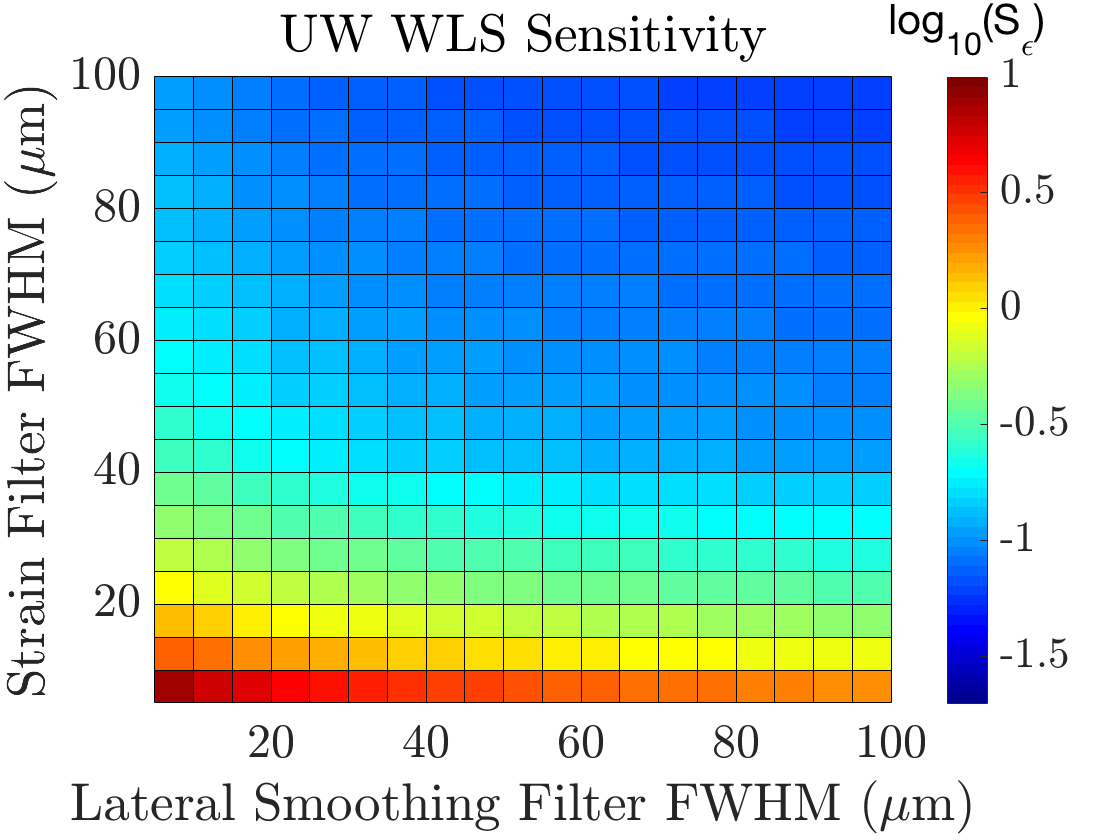
\includegraphics[width=\textwidth]{appendix_figs/wls_sensitivity.png}
	\end{subfigure}
	\begin{subfigure}{0.49\textwidth}
    		\centering
	        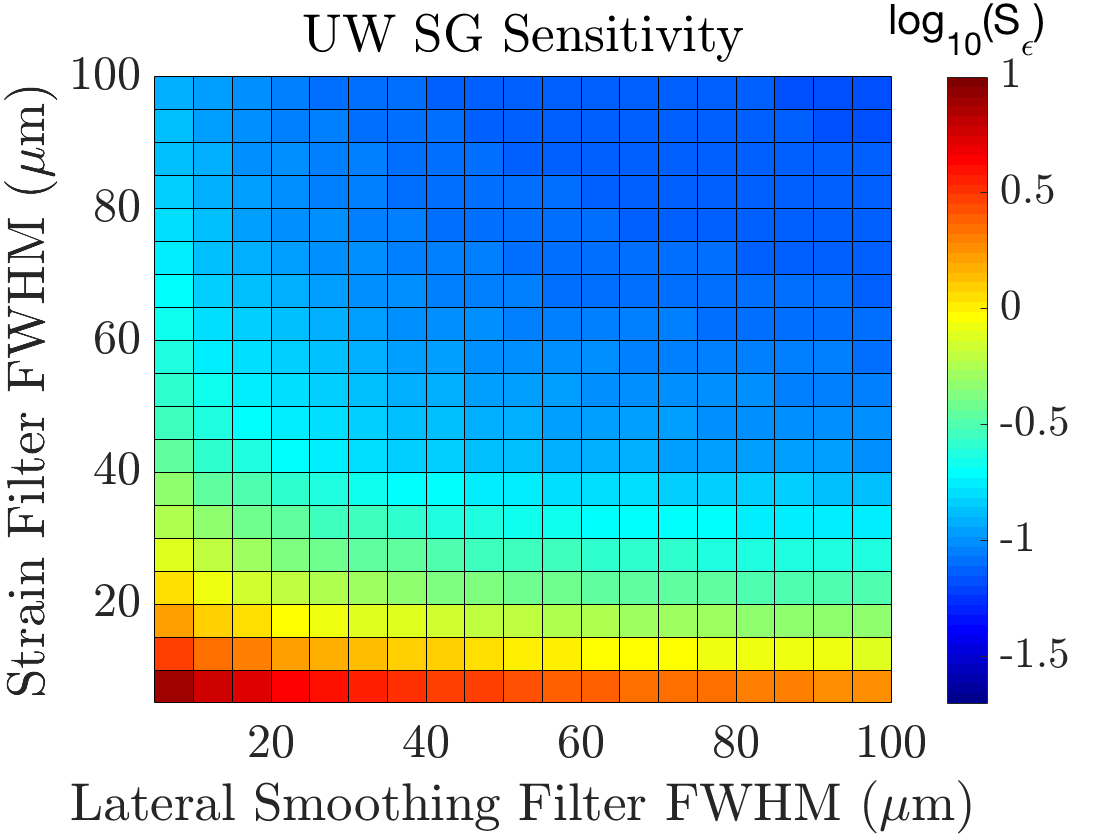
\includegraphics[width=\textwidth]{appendix_figs/uwsg_sensitivity.png}
	\end{subfigure}
    	\\
    	\begin{subfigure}{0.49\textwidth}
    		\centering
	        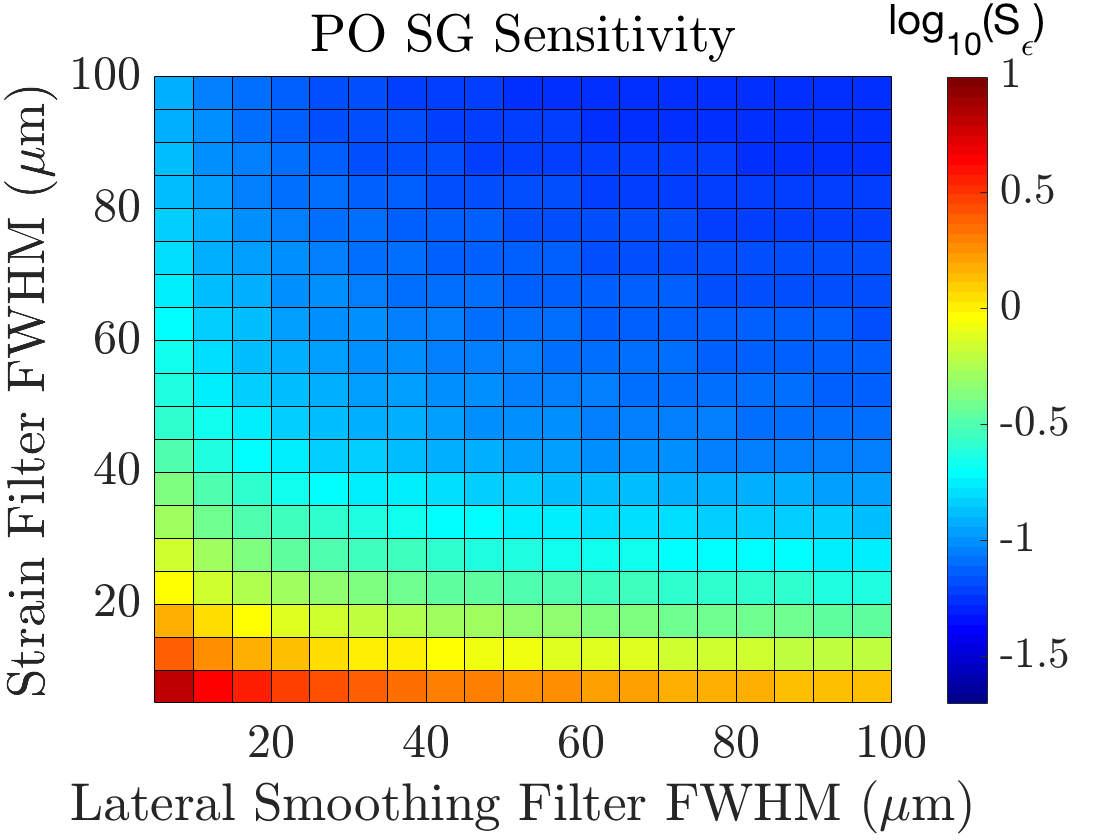
\includegraphics[width=\textwidth]{appendix_figs/posg_sensitivity.png}
	\end{subfigure}
    	\begin{subfigure}{0.49\textwidth}
    		\centering
	        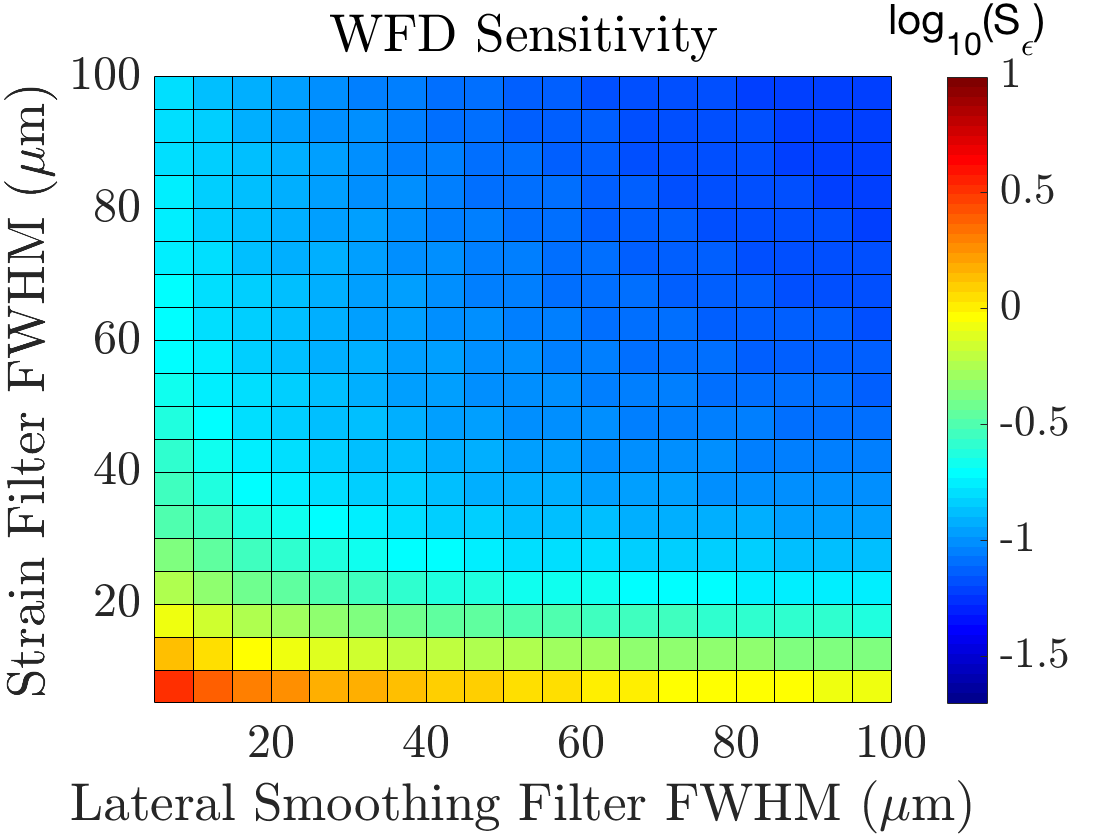
\includegraphics[width=\textwidth]{appendix_figs/wfd_sensitivity.png}
	\end{subfigure}
    	\\
    	\begin{subfigure}{0.49\textwidth}
    		\centering
        	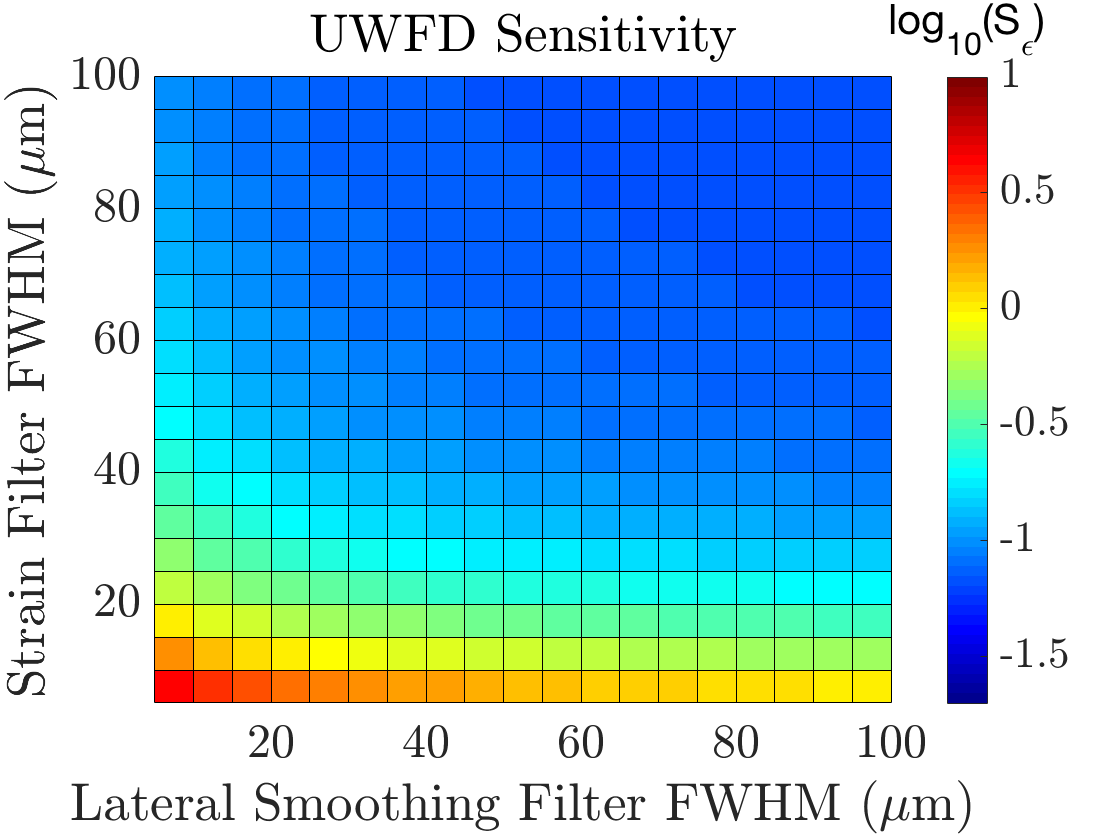
\includegraphics[width=\textwidth]{appendix_figs/uwfd_sensitivity.png}
	\end{subfigure}
	\begin{subfigure}{0.49\textwidth}
    		\centering
	        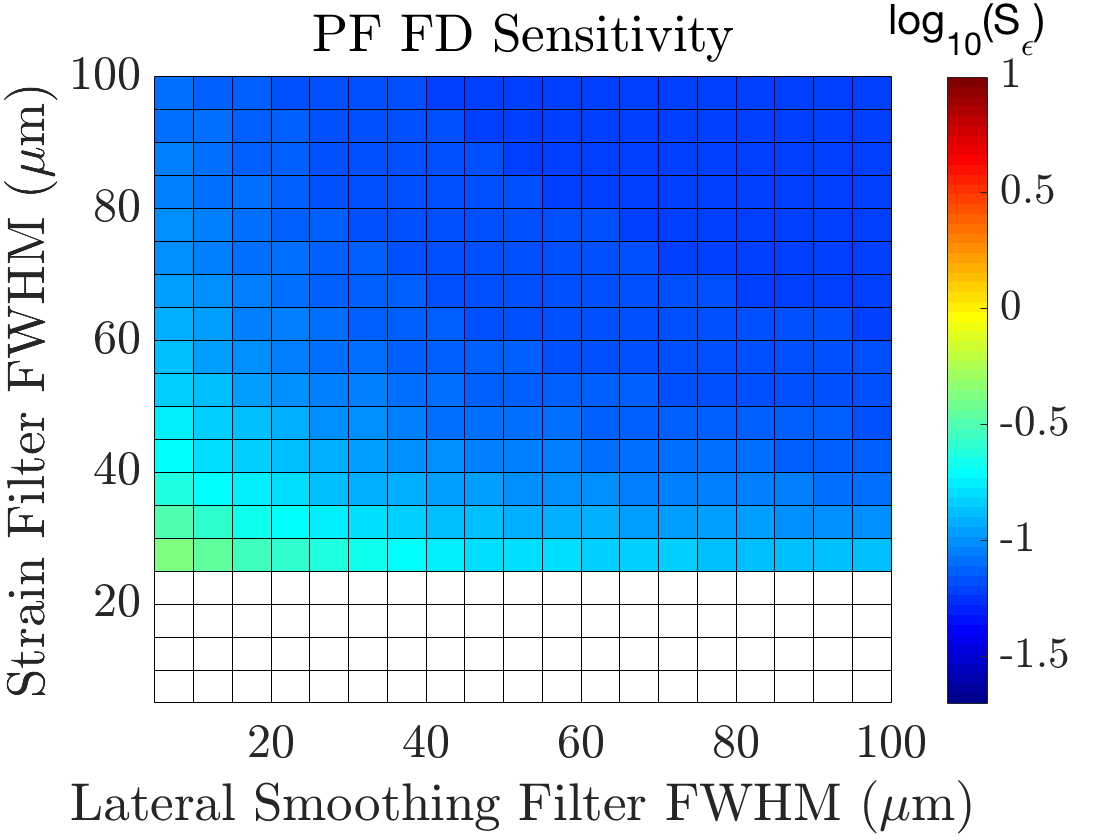
\includegraphics[width=\textwidth]{appendix_figs/pffd_sensitivity.png}
    	\end{subfigure}
    	\caption{Log sensitivity heat maps for different strain and lateral smoothing filter \ac{fwhm} resolutions. Regions that are red correspond to worse sensitivity (higher values).}
	\label{sensitivity_heatmaps}	
\end{figure}

